%
% File: chap01.tex
% Author: Victor F. Brena-Medina
% Description: Introduction chapter where the biology goes.
%
\let\textcircled=\pgftextcircled
\chapter{Literature Review}
\label{chap:conclusion}
\paragraph{}

\section{Previous Work}
\paragraph{}

Jonathan Rose[2] has done some work on architecting FPGAs. He first develops concepts of island-style FPGAs and then demonstrates different routing methods. He further provides a software tool to automate the layout generation of an FPGA by iteratively placing tiles of a CLB and Switch Matrix. This tool isnot compatible with modern PDKs and the tool isn't even available publically. Only a final netlist of their FPGA is provided which is not easy to scale or modify. 
[3] analyzes various parameters of an island-style FPGA architecture from theoretical derivations of area and delay but the models are approximate. The various area models used in the derivations are shown in Fig. 2.1. Equations 1.1 to 1.4 give approximations of total area required to layout an FPGA using these approximations. 

\begin{figure}[h]
\centering
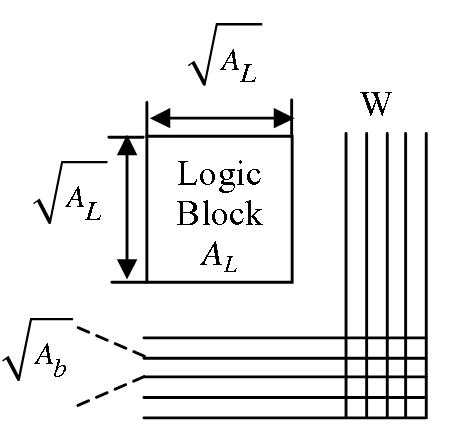
\includegraphics[width=0.3\linewidth]{area_model.png}
\caption{Area model used in [3]}
\label{fig:Figure}
\end{figure}

\begin{equation}
A_{Tile} = A_L + A_R
\end{equation}
\begin{equation}
A_L^K = A_b\cdot2^K + A_f
\end{equation}
\begin{equation}
A_R^K = A_b{\cdot}W_K^2 + 2\cdot\sqrt{A_b}\cdot\sqrt{A_L^K}{\cdot}W_K
\end{equation}
\begin{equation}
A_{Total}^K = A_{Tile}^K{\cdot}N_K = {(\sqrt{A_b}{\cdot}W_K + \sqrt{A_L^K})}^2{\cdot}N_K
\end{equation}

$A_{Tile}$ : Area of a single tile \hfill
$A_L$ : Area of Logic Block per tile \hfill
$A_R$ : Area of Routing per tile \hfill
$A_b$ : Area of an SRAM cell \hfill
$K$ : Number of Inputs to one CLB \hfill
$N_K$ : Number of tile required with K-size CLBs \hfill

\begin{figure}[h]
\centering
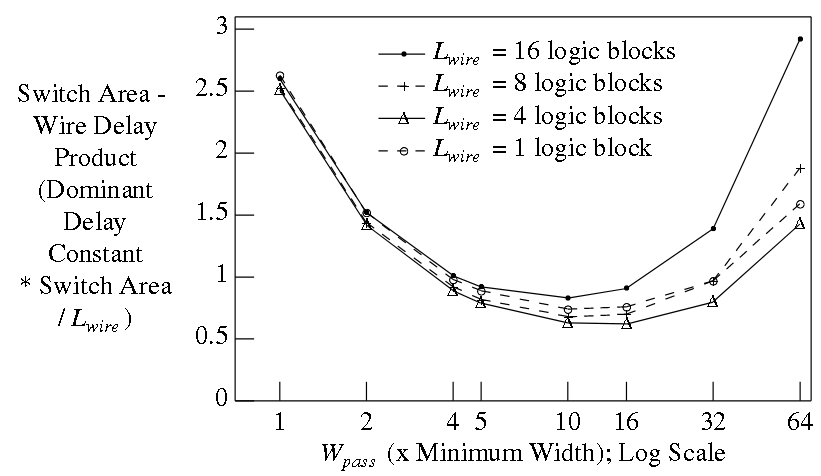
\includegraphics[width=0.9\linewidth]{previous_work.png}
\caption{Sizing pass transistors of the switch matrices[5]}
\label{fig:Figure}
\end{figure}

The FPGA research community has developed the VTR Project[4]. VTR(Verilog to Routing) is a tool chain which facilitates FPGA architecture research. The tool needs a description of the FPGA architecture in a special pre-defined XML format along with the Verilog file which is to be implemented on the FPGA. The tool will first determine the grid size and routing width needed to implement the circuit and then perform coarse and fine grained routing to produce a netlist. This tool is not very well supported in the schematic level circuit simulation softwares as well as layout tools. 

[5] proposes methodologies to size interconnect circuits as shown in Fig. 2.2 but does not consider the effect of CLB circuit on the sizing by assuming a buffer in between which limits it to a first hand approximation. We use these suggested values as a starting point in the project.
